\documentclass[a4 paper]{article}
\usepackage[inner=2.0cm,outer=2.0cm,top=2.5cm,bottom=2.5cm]{geometry}
\usepackage{setspace}
\usepackage[rgb]{xcolor}
\usepackage{verbatim}
\usepackage{subcaption}
\usepackage{amsgen,amsmath,amstext,amsbsy,amsopn,tikz,amssymb}
\usepackage{fancyhdr}
\usepackage[colorlinks=true, urlcolor=blue,  linkcolor=blue, citecolor=blue]{hyperref}
\usepackage[colorinlistoftodos]{todonotes}
\usepackage{rotating}
\usepackage{booktabs}
\newcommand{\ra}[1]{\renewcommand{\arraystretch}{#1}}

\newtheorem{thm}{Theorem}[section]
\newtheorem{prop}[thm]{Proposition}
\newtheorem{lem}[thm]{Lemma}
\newtheorem{cor}[thm]{Corollary}
\newtheorem{defn}[thm]{Definition}
\newtheorem{rem}[thm]{Remark}
\numberwithin{equation}{section}

\newcommand{\homework}[6]{
   \pagestyle{myheadings}
   \thispagestyle{plain}
   \newpage
   \setcounter{page}{1}
   \noindent
   \begin{center}
   \framebox{
      \vbox{\vspace{2mm}
    \hbox to 6.28in { {\bf CSE 211:~Discrete Mathematics \hfill {\small (#2)}} }
       \vspace{6mm}
       \hbox to 6.28in { {\Large \hfill #1  \hfill} }
       \vspace{6mm}
       \hbox to 6.28in { {\it Instructor: {\rm #3} \hfill  {\rm #5} \hfill  {\rm #6}} \hfill}
       \hbox to 6.28in { {\it Assistant: #4  \hfill #6}}
      \vspace{2mm}}
   }
   \end{center}
   \markboth{#5 -- #1}{#5 -- #1}
   \vspace*{4mm}
}

\newcommand{\problem}[2]{~\\\fbox{\textbf{Problem #1}}\hfill (#2 points)\newline\newline}
\newcommand{\subproblem}[1]{~\newline\textbf{(#1)}}
\newcommand{\D}{\mathcal{D}}
\newcommand{\Hy}{\mathcal{H}}
\newcommand{\VS}{\textrm{VS}}
\newcommand{\solution}{~\newline\textbf{\textit{(Solution)}} }

\newcommand{\bbF}{\mathbb{F}}
\newcommand{\bbX}{\mathbb{X}}
\newcommand{\bI}{\mathbf{I}}
\newcommand{\bX}{\mathbf{X}}
\newcommand{\bY}{\mathbf{Y}}
\newcommand{\bepsilon}{\boldsymbol{\epsilon}}
\newcommand{\balpha}{\boldsymbol{\alpha}}
\newcommand{\bbeta}{\boldsymbol{\beta}}
\newcommand{\0}{\mathbf{0}}


\begin{document}
\homework{Homework \#3}{Due: 03/01/22}{Dr. Zafeirakis Zafeirakopoulos}{Gizem S\"ung\"u}{}{}
\textbf{Course Policy}: Read all the instructions below carefully before you start working on the assignment, and before you make a submission.
\begin{itemize}
\item It is not a group homework. Do not share your answers to anyone in any circumstance. Any cheating means at least -100 for both sides. 
\item Do not take any information from Internet.
\item No late homework will be accepted. 
\item For any questions about the homework, send an email to gizemsungu@gtu.edu.tr
\item The homeworks (both latex, pdf and/or source code files in a zip file) will be
submitted into the course page of Teams.
\item The latex, pdf or source code and zip files of the homeworks should be saved as
"StudentId".$\{$tex, pdf, c, py, cpp, java, zip$\}$.
\item If the answers of the homeworks have only calculations without any formula or any explanation -when needed- will get zero.
\end{itemize}

\problem{1: Relations}{20}
Let $\mathbb{Z}$ be the set of all integers. Define relation R on $\mathbb{N}$ as follows.
\begin{equation*}
	\forall a, b \in \mathbb{N}, (a, b) \in R \text{ iff } \exists i \in \mathbb{Z},  \frac{a}{b} = 2^i
\end{equation*}
Prove that R is an equivalence relation. Show your work step by step.
\newline
\textbf{To R be an equivalence relation, it has to provide this properties:}
\begin{itemize}
\item Reflexivity
\textbf{(a,a) must be one of the element of the set. So, $\frac{a}{a}$ = $2^i$ $\Rightarrow$ i = 0, i provides the condition: i $\in$ $\mathbb{Z}$. So, it is reflexive.}
\item Symmetry
\textbf{If (a,b) is one of the element of the set, there must be an element such as (b,a) to be symmetry. So, $\frac{a}{b}$ = $2^k$ $\land$ $\exists$ k $\in$ $\mathbb{Z}$, for element (b,a) $\frac{b}{a}$ = $2^{-k}$, k $\in$ $\mathbb{Z}$ $\Rightarrow$ -k $\in$ $\mathbb{Z}$. So, it is symmetric.}
\item Transitivity
\textbf{if (a,b) and (b,c) are elements of the set, there must be an element such as (a,c). So, $\frac{a}{b}$ = $2^k$ $\land$ $\frac{b}{c}$ = $2^l$ $\Rightarrow$ $\frac{a}{c}$ = $2^{k+l}$. If k $\land$ l $\in$ $\mathbb{Z}$, k+l $\in$ $\mathbb{Z}$. So it is transitive.}
\end{itemize}
\textbf{As the result; it provides all of the condition, so it is an equivalence relation.}
\newline
\problem{2: Relations}{15}
Define he relation R on $\mathbb{N}$ as 
\begin{equation*}
	\forall c, d \in \mathbb{N}, (c, d) \in R \text{ iff } c+d \text{ is even.}
\end{equation*}
\subproblem{a} Prove that R is an equivalence relation.
\subproblem{b} How many equivalence classes does R have?
\newline
\textbf{a) to R be an equivalence relation, it has to provide this properties:}
\begin{itemize}
\item Reflexivity
\textbf{(a,a) must be one of the element of the set. So, a+a = 2a. 2a can be divided by 2. So, it is reflexive.}
\item Symmetry
\textbf{If (a,b) is one of the element of the set, there must be an element such as (b,a) to be symmetry. So,for element (a,b): a+b = 2k (b,a). For element (b,a): b+a = 2k. So, it is symmetric.}
\item Transitivity
\textbf{if (a,b) and (b,c) are elements of the set, there must be an element such as (a,c). So, a+b = 2k $\land$ b+c = 2l $\Rightarrow$ a+c = (2k-b+2l-b) = 2(k+l-b) which is divisible by 2. So it is transitive.}
\end{itemize}
\textbf{b) [1] =  \{1, 3, 5, 7...\}, [2] = \{0. 2, 4, 6, 8...\}, [3] = \{1, 3, 5, 7...\}, [4] = \{0, 2, 4, 6, 8...\}. So there are two distinct classes. One for even numbers, one for odd numbers.}
\newline
\problem{3: Relations}{10}
Let R and S be two relations both on A. Show that
\subproblem{a} If R and S are both reflexive, is R $\cap$ S also reflexive?
\newline
\textbf{Let (a,b) is one of the element of the set R $\cap$ S. If (a,b) is one of the element of the set R $\cap$ S, (a,b) is one of the elements of both R and S sets. (a,a) and (b,b) are one of the elements of R and S sets because they are reflexive. (a,a),(b,b) $\in$ R $\land$ (a,a),(b,b) $\in$ S $\Rightarrow$ (a,a),(b,b) $\in$ R $\cap$ S. So R $\cap$ S is reflexive.}
\subproblem{b} If R and S are both symmetric, is R $\cap$ S also symmetric?
\newline
\textbf{Let (a,b) is one of the element of the set R $\cap$ S. If (a,b) is one of the element of the set R $\cap$ S, (a,b) is one of the elements of both R and S sets. (a,b) and (b,a) are one of the elements of R and S sets because they are symmetric. (a,b),(b,a) $\in$ R $\land$ (a,a),(b,b) $\in$ S $\Rightarrow$ (a,b),(b,a) $\in$ R $\cap$ S. So R $\cap$ S is symmetric.}
\subproblem{c} If R and S are both transitive, is R $\cap$ S also transitive?
\newline
\textbf{Let (a,c) is one of the element of the set R $\cap$ S. If (a,c) is one of the element of the set R $\cap$ S, (a,c) is one of the elements of both R and S sets. (a,b) and (b,c) are one of the elements of R and S sets because they are reflexive. (a,b),(b,c) $\in$ R $\land$ (a,b),(b,c) $\in$ S $\Rightarrow$ (a,b),(b,c) $\in$ R $\cap$ S. So R $\cap$ S is transitive.}
\newline
Note: Of course, yes or no answers are not acceptable. Show your work briefly.
\newpage
\problem{4: Relations}{15}
Give a poset that has
\subproblem{a} a minimal element but no maximal element.
\textbf{(N, $\le$): minimal element is 0 but not have maximal element.}
\subproblem{b} a maximal element but no minimal element.
\textbf{(Z$_{\le0}$, $\le$): maximal element is 0 but not have minimal elements.} 
\subproblem{c} neither a maximal nor a minimal element.
\textbf{(Z, $\le$): it goes to forever both sides.}
\problem{5: Relations}{15}
Suppose that (S, $\preccurlyeq_1$) and (T , $\preccurlyeq_2$) are posets. Show that
(S $\times$ T , $\preccurlyeq$) is a poset where (s, t) $\preccurlyeq$ (u, v) if and only if
s $\preccurlyeq_1$ u and t $\preccurlyeq_2$ v. Show your work in details. 
\newline
\textbf{If there is a relation such as s $\preccurlyeq_1$ u, s and u are elements of S;
if there is a relation such as  t $\preccurlyeq_2$ v, t and v are elements of T. S x T = \{(s,t), (s,v), (u,t), (u,v)\}. Therefore there is a relation (s,t) $\preccurlyeq$ (u,v) between them.}

\problem{6: Relations}{10}
Answer these questions for the partial order represented by this Hasse diagram.
\begin{figure}[htb]
	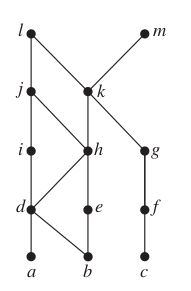
\includegraphics[scale=0.5]{hasse.png}
\end{figure}
\subproblem{a} Find the maximal elements.
\textbf{: l and m}
\subproblem{b} Find the minimal elements.
\textbf{: a, b and c}
\subproblem{c} Is there a greatest element?
\textbf{: No, there is not greatest elements because there is no unique maximal element.}
\subproblem{d} Is there a least element?
\textbf{: No, there is not least elements because there is no unique minimal element.}
\subproblem{e} Find all upper bounds of $\{a, b, c\}$.
\newline
\textbf{\{a, b, c, d, e, f, g, h, i, j, k, l, m\}}
\newline
\textbf{\{a, b, c\}}
\newline
\textbf{\{+aRa, -aRb, -aRc, +aRd, -aRe, -aRf, -aRg, +aRh, +aRi, +aRj, +aRk, +aRl, +aRm\}}
\newline
\textbf{\{-bRa, +bRb, -bRc, +bRd, +bRe, -bRf, -bRg, +bRh, +bRi, +bRj, +bRk, +bRl, +bRm\}}
\newline
\textbf{\{-cRa, -cRb, +cRc, -cRd, -cRe, +cRf, +cRg, -cRh, -cRi, -cRj, +cRk, +cRl, +cRm\}}
\newline
\textbf{Upper bounds: \{k, l, m\}}
\subproblem{f} Find the least upper bound of  $\{a, b, c\}$, if it exists.
\textbf{Least upper bound is \{k\}. Because it is closest.}
\subproblem{g} Find all lower bounds of  $\{f, g, h\}$.
\newline
\textbf{\{-aRf, -aRg, -aRh\}}
\newline
\textbf{\{-bRf, -bRg, +bRh\}}
\newline
\textbf{\{+cRf, +cRg, -cRh\}}
\newline
\textbf{\{-dRf, -dRg, +dRh\}}
\newline
\textbf{\{-eRf, -eRg, +eRh\}}
\newline
\textbf{\{+fRf, +fRg, -fRh\}}
\newline
\textbf{\{-gRf, +gRg, -gRh\}}
\newline
\textbf{\{-hRf, -hRg, +hRh\}}
\newline
\textbf{\{-iRf, -iRg, -iRh\}}
\newline
\textbf{\{-jRf, -jRg, -jRh\}}
\newline
\textbf{\{-kRf, -kRg, -kRh\}}
\newline
\textbf{\{-lRf, -lRg, -lRh\}}
\newline
\textbf{\{-mRf, -mRg, -mRh\}}
\newline
\textbf{There is no lower bound.}
\subproblem{h} Find the greatest lower bound of  $\{f, g, h\}$, if it exists.
\textbf{It it not exist.}
\newpage
\problem{7: Graphs}{10}
Determine whether the directed graph shown has an Euler circuit. Construct an Euler circuit if one exists. If no Euler circuit exists, determine whether the directed graph has an Euler path. Construct an Euler path if one exists.
\subproblem{a}
\begin{figure}[htb]
	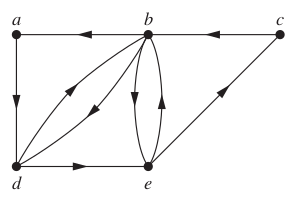
\includegraphics[scale=0.5]{euler.png}
	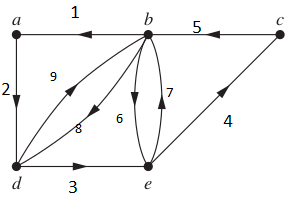
\includegraphics[scale=0.65]{myeuler.png}
\newline
\textbf{Euler circuit exist.}
\end{figure}
\subproblem{b}
\begin{figure}[h]
	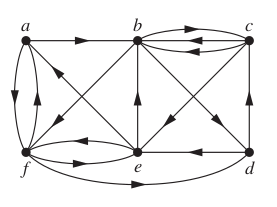
\includegraphics[scale=0.5]{euler2.png}

\end{figure}

\problem{8: Graphs}{25}
Remember graph coloring problem in the problem session.
\subproblem{a} Draw the graph of the following code block.
\subproblem{b} Explain how you represent the components of the code in graph coloring problem. 
\subproblem{c} What is the minimum number of registers that you need to compile the code? Show which variables can be in the same register.
\textbf{We need c and f until line 8, need a until line 7, need b until line 6, need d until line 5. So we need three register for a, b and c. We need one more register for d because we cannot use register of a, b or c. We do not need a register for e because we can use register d we do not need anymore it. We do not need a register for f either, because we can use register of d again. So the code is compilable with just 4 register. }

\begin{itemize}
	\item[Line 1:] a = 3
	\item[Line 2:] b = 6
	\item[Line 3:] c = 4
	\item[Line 4:] d = b + c
	\item[Line 5:] e = d + a
	\item[Line 6:] if e $<$ 4 then f = 4 $\times$ b   
	\item[Line 7:] else then f = 6 $\times$ a
	\item[Line 8:] d = f - c
\end{itemize}

\problem{9: Graphs}{10}
Draw graphs which are given in adjaceny matrices as follows. Explain if these graphs are isomorphic?


\begin{equation*}
G_1 = \begin{bmatrix} 
0 & 1 & 0 & 1\\
1 & 0 & 0 & 1\\
0 & 0 & 0 & 1\\
1 & 1 & 1 & 0
\end{bmatrix}\mbox{ ~    ~ }     
G_2 = \begin{bmatrix}
0 & 1 & 1 & 1\\
1 & 0 & 0 & 1\\
1 & 0 & 0 & 1\\
1 & 1 & 1 & 0
\end{bmatrix}
\end{equation*} 
\textbf{G1: }
\begin{figure}[htb]
\textbf{G2: }
	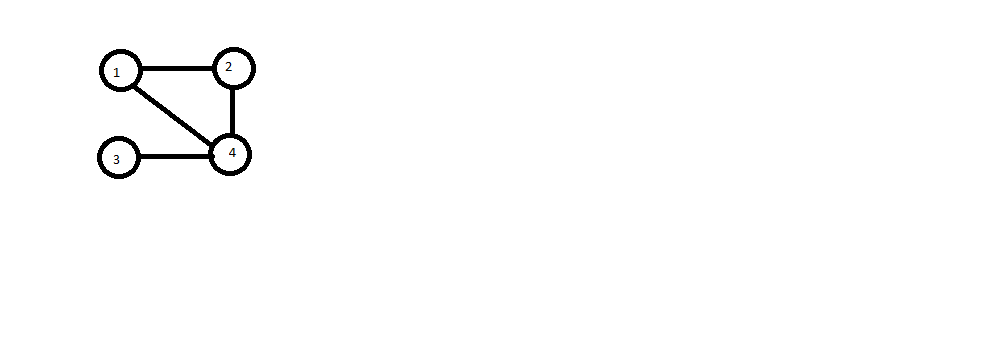
\includegraphics[scale=0.65]{matrix1.png} 
	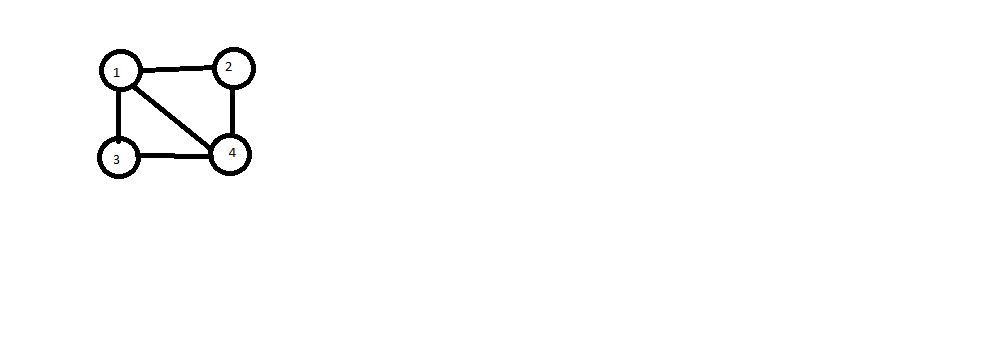
\includegraphics[scale=0.65]{matrix2.png}
\end{figure}
\end{document} 
